\documentclass[a4paper, 12pt]{article}
\usepackage{apacite}
\usepackage{graphicx}
\usepackage[T1]{fontenc}
\usepackage[utf8]{inputenc}
\usepackage{mathptmx}
\usepackage{enumerate}
\usepackage[margin=0.5in]{geometry}
\usepackage{lipsum}

\renewcommand{\baselinestretch}{1.0}

\newcommand\nd{\textsuperscript{nd}\xspace}
\newcommand\rd{\textsuperscript{rd}\xspace}
\newcommand\nth{\textsuperscript{th}\xspace} %\th is taken already

\setlength\parindent{0pt} % set paragraph indent to zero

% fill up your name, ID and paper title here
\author{
LOA TAT ANN \quad 1221304731 \quad  contribution1 \\
YU BUI XUAN \quad 241UC24121\quad contribution2\\
MOHAMAD SYAMEL BIN MOHAMAD KARID \quad 1221309130 \quad contribution3\\
% Student Name4 \quad Student ID4 \quad contribution4\\
}
\title{Comparison of Machine Learning Methods Used for Detecting DDoS Attacks in Performance and Accuracy}

\begin{document}
\maketitle

\begin{abstract}

\end{abstract}


\section{Introduction}
As the world has become increasingly connected, the rapid evolution of network technologies has also led to cyberattacks becoming much more common and harder to contain. This includes DDoS (Distributed Denial of Service) attacks, which try to disrupt network services by overloading a network with malicious traffic (bots) and denying normal system access. \citeA{1} Such attacks can even affect and suffer the largest companies such as the online retailer and cloud service provider Amazon in 2020, where a DDoS attack was detected on its services with a recorded access rate of 2.3 Tbps, and in 2016, where a DDoS attack disrupted a major DNS infrastructure provider which caused several major networks like Twitter (X) and PayPal became inaccessible to users for 3 hours. \citeA{1} 

There are several ways DDoS attacks the host system, including sending malicious traffic at a slow pace to a target (low-rate attacks), using a high amount of packets to compromise the system (high-rate) attacks, exploiting network protocol vulnerabilities to use up resources (protocol exploitation), and substituting the IP address of the victim with the attacker's (reflection-amplification). \citeA{1} 

To prevent such attacks, various methods are also developed to detect, prevent and mitigate such attacks from harming the system. One such example involves machine learning as they have good performance on network anomaly detection, and it can be adapted to deal with new threats. \citeA{3}

\section{Problem Statement}
Researchers use several different test methods to detect DDoS attacks with machine learning. The main methods are supervised and unsupervised methods. Supervised methods involve a physical network in a lab-based environment where the attacker and the victim exist in the same network and all tests are controlled scientifically. On the flip side, unsupervised methods test the system with real-world networks. The data collected from such methods are analyzed based on their characteristics. \citeA{1}

With the development of various methods available, it can be difficult to determine the best method for detecting DDoS networks for a system, as they have different needs and constraints. Furthermore, each detection scenario is different, as they do not always have the same situation and attributes as others. 

This research aims to compare various machine learning models by comparing their accuracy, performance and efficiency of the models regarding detecting DDoS attacks, and determine which methods are suitable for different environments. 

\section{Methodology}
\subsection{TPAAD}
The TPAAD two-phase authentication system, written by Najmun Nisa, Adnan Shahid Khan, Zeeshan Ahmad, and Johari Abdullah, explains a new method that utilizes machine learning algorithms such as Support Vector Machine (SVM) and K-Nearest Neighbors (KNN) to detect DDoS attacks on Software-Defined Networks (SDNs) efficiently. The system also filters incoming packets to detect and stop malicious traffic without host deactivation and affecting normal network connectivity. \citeA{3} The detection for the system works by utilizing two different modules, which are for detecting threats and mitigating the risks. 

The detection module continuously monitors the network to identify abnormal traffic. Then packet filtration techniques used by the mitigation module are used to split network traffic to contain and find suspicious activity with machine learning models referring to a predefined dataset (CICDoS 2017). After that, the system employs a tunnelling mechanism to block or reroute malicious traffic ensuring normal network activity is unaffected. \citeA{3}

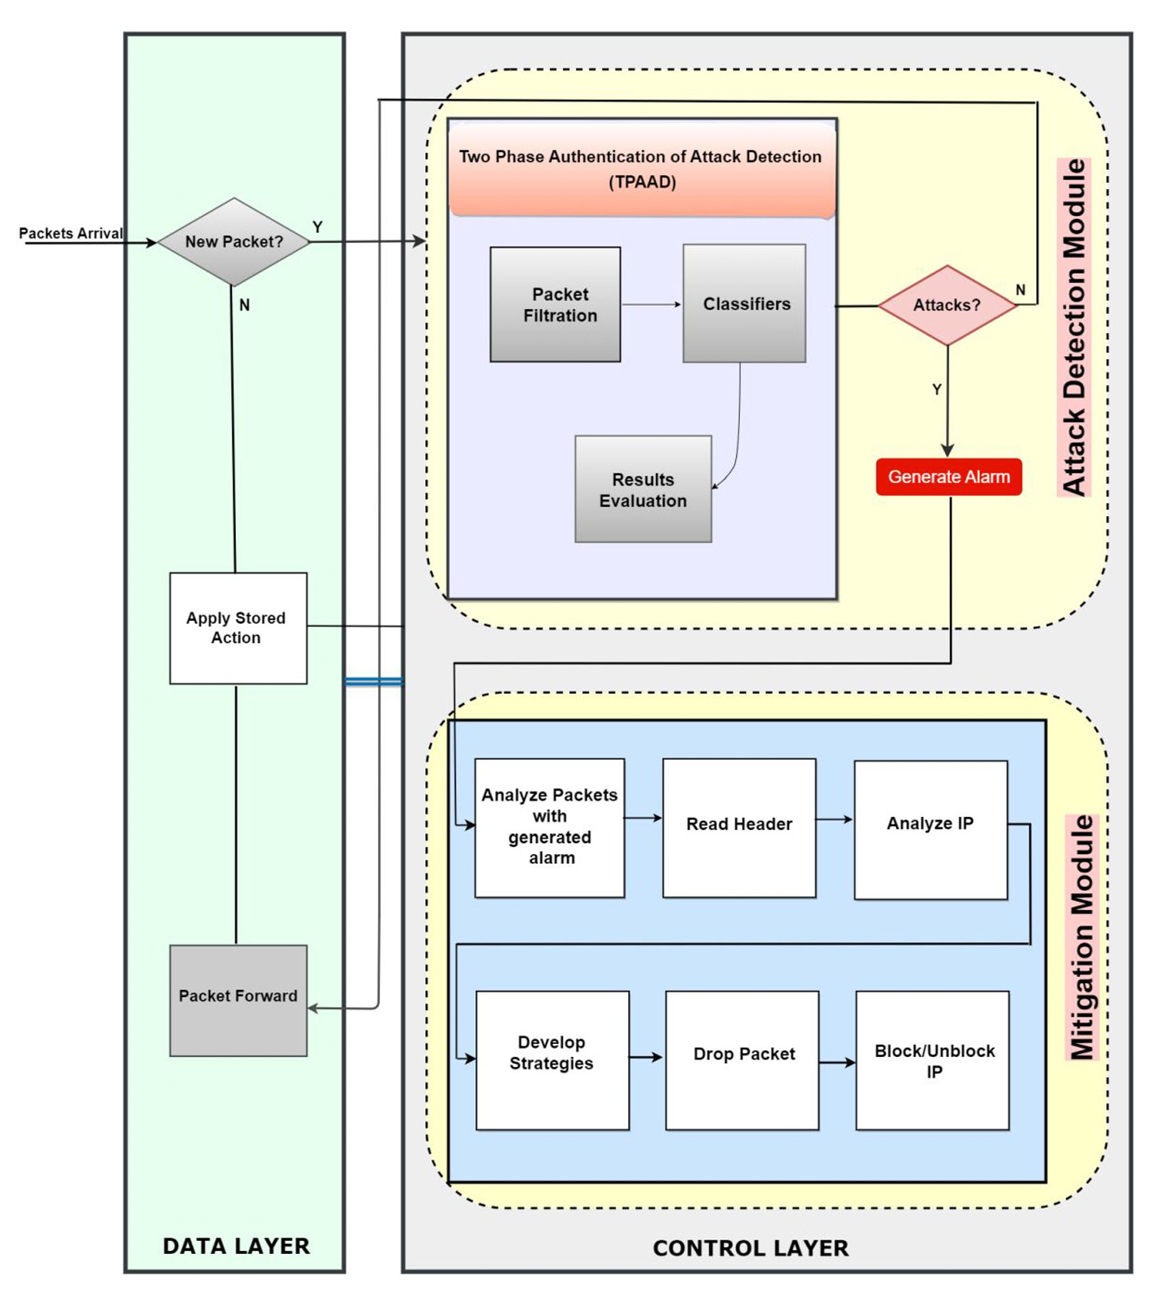
\includegraphics[scale=0.3]{IMG_0249.jpeg} \\
Fig 1: Diagram for the TPAAD system. \citeA{3}

\subsection{Flexible SDN-Based Architecture}
Low-rate DDoS attacks are more challenging to contain as they target network protocols such as TCP without overloading the system. Because of this, they are harder to detect as they are "integrated" with legitimate network traffic and are difficult to detect and report, and data for such attacks are harder to extract. Hence, the paper proposes a novel modular system architecture to detect such incidents with machine learning techniques. \citeA{4}

The methods used by the system includes Support Vector Machines (SVM), Random Forest (RF), K-Nearest Neighbors (KNN), and Multi-Layer Perceptron (MLP).  Important criteria including computing efficiency, false positive rate, and detection accuracy are used to evaluate each method. These models are trained on the CIC DoS 2017 dataset, widely used in DDoS detection research, and the most effective strategy for real-time network protection is determined by analyzing their capacity to distinguish between malicious and legitimate traffic with accuracy. \citeA{4}

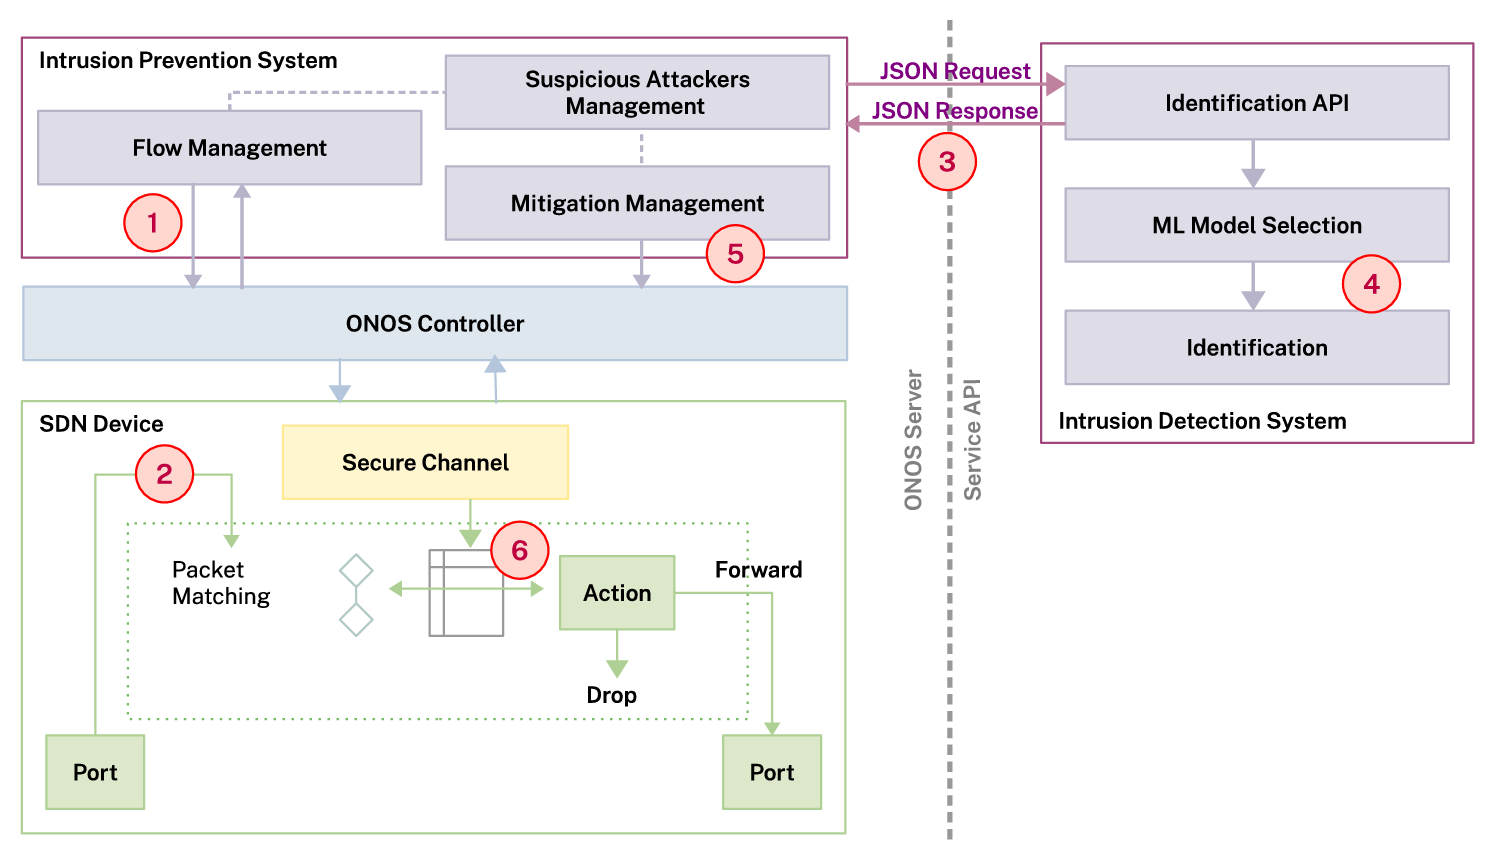
\includegraphics[scale=0.3]{IMG_0250.jpeg} \\
Fig 2: Diagram for the SDN-based architecture system. \citeA{4}

\subsection{ML-DDoSnet} 
The methodology in this study focuses on using eight machine learning algorithms to detect and classify Distributed Denial of Service (DDoS) attacks in IoT environments. A variety of models are employed, such as Decision Tree (DT), Random Forest (RF), K-Nearest Neighbors (KNN), Support Vector Machine (SVM), Multilayer Perceptron (MLP), Linear Discriminant Analysis (LDA), and two deep learning approaches: Long Short-Term Memory (LSTM) and Bidirectional LSTM (BiLSTM). The study utilizes the NSL-KDD dataset for training and testing, which includes labelled data (normal or anomalous). Key steps in enhancing model performance by reducing redundant features are feature extraction and selection. Metrics like accuracy, precision, recall, and F1 score are used to compare the models. BiLSTM performs better than the others in terms of identifying DDoS assaults with greater accuracy and reducing false positives. \citeA{5}

\subsection{GRU-LM and Word2vec}
The study proposes a hybrid deep learning method to mitigate DDoS attacks in real-time within mobile networks using Word2vec and a Gated Recurrent Unit Language Model (GRU-LM). The method involves the use of Light Gradient Boosting Machine (LGBM) to detect DDoS attacks with 100\% accuracy. Natural language processing (NLP) techniques are used to enhance the model. Word2vec is used to embed Python source code, and GRU is used to predicting the next word in the code sequence. Compared to conventional GRU and LSTM models, this method effectively reduces computational time and memory utilization, which makes it appropriate for real-time DDoS detection in mobile situations. \citeA{6}

\section{Results}

\subsection{TPAAD} 
According to the tests, the TPAAD system recorded a 99.56\% accuracy on detecting DDoS attacks when testing with the CICDoS 2017 dataset on a controlled environment running on an Ubuntu VM on VMWare and an SDN setup created via Mininet and the RYU controller. \citeA{3} Besides that, the CPU utilization for the system was recorded at 

\subsection{Flexible SDN-Based Architecture}

\subsection{ML-DDoSnet}

\subsubsection{GRU-LM and Word2vec}

\section{Discussions}
\subsection{Overview Of The Methods}
\subsection{Analysis of Individual Methods}
%pros and cons, limitation
\subsubsection{TPAAD}
\subsubsection{Flexible SDN-Based Architecture}
\subsubsection{ML-DDoSnet}
\subsubsection{GRU-LM and Word2vec}
\subsection{Contribution Of The Research}

\section{Conclusion}
% Discussions include but not limited to:
%\begin{enumerate}[(a)]
%\item Pros and cons of the method/algorithm used,
%\item limitation of the method/algorithm,
%\item contribution of the research.
% \end{enumerate}
%Conclusion of the work presented in the reviewed research papers.

There are some pros and cons of such methods. For example, The TPAAD system records good accuracy in detecting threats while using minimal resources through efficient network filtering and traffic management. Also, the system can dynamically adjust to other threats to reduce disruptions. However, the system has the potential for delays due to the processing of traffic, as well as a highly complex system which increases the difficulty of deployment. Besides that, the system's reliability is highly dependent on dataset quality which could increase the false negatives of the system if an inadequate dataset is used. \citeA{3}

Every problem must have a solution, but the best solution depends on the use case and other factors. DDoS attacks are still a major concern for Internet network services, and the challenge remains. Despite this, machine learning will still need more work to have the best results in detecting threats, in a balanced approach that combines cost and performance equally. As the need for cybersecurity and machine learning evolves, the collaboration of all parties involved will be crucial to protecting our networks from DDoS attacks. 

\section{Future work}
Despite the work, the report still faces some issues while creeating.

\section{Paper 2: A Flexible SDN-Based Architecture for Identifying and Mitigating Low-Rate DDoS Attacks Using Machine Learning}

\subsection{Methodology}
The study compares various machine learning methods for DDos attack detection, focusing on their performance and accuracy. The methods include Support Vector Machines (SVM), Random Forest (RF), K-Nearest Neighbors (KNN), and Multi-Layer Perceptron (MLP).  Important criteria including computing efficiency, false positive rate, and detection accuracy are used to evaluate each method. These models are trained on the CIC DoS 2017 dataset, widely used in DDoS detection research, and the most effective strategy for real-time network protection is determined by analyzing their capacity to distinguish between malicious and legitimate traffic with accuracy. \citeA{4}

\subsection{Results}

\section{Paper 3: DDoS attacks and machine-learning-based detection methods: A survey and taxonomy}

\subsection{Methodology}
The research compares various machine learning methods for DDos attack detection, focusing on their performance and accuracy categorizes machine learning-based detection methods into three groups: supervised, unsupervised, and hybrid approaches. For classification applications where labeled datasets are available, supervised techniques like Random Forest (RF), Support Vector Machine (SVM), and Decision Tree (DT) are commonly utilized. These models are often trained on two datasets, CICDDoS2019 and KDDCup99, offering a variety of attack scenarios for evaluation. Unsupervised algorithms such as DBSCAN and K-Means cluster traffic patterns to detect anomalies without prior labels, while hybrid approaches combine both techniques to improve detection accuracy. When performance parameters like accuracy, precision, recall, and false positive rate are used to assess various techniques, it becomes clear that, in many cases, RF and SVM work well, with detection rates reaching 99\% in specific scenarios. \citeA{1}

\subsection{Results}

\section{Paper 4: Machine Learning and Deep Learning Techniques for Distributed Denial of Service Anomaly Detection in Software Defined Networks—Current Research Solutions}

\subsection{Methodology}
This research offers a comparative analysis of both Machine Learning (ML) and Deep Learning (DL) techniques for detecting Distributed Denial of Service (DDoS) attacks within Software Defined Networks (SDNs). Network traffic data is processed and analyzed using supervised, unsupervised, and hybrid learning models as the main techniques. The study uses prominent datasets, including CICDDoS2019 and CSE-CIC-IDS2018, to train and test several models, such as Support Vector Machine (SVM), Random Forest (RF), and Convolutional Neural Networks (CNN). Performance metrics like accuracy, precision, recall, and F1 score are used to evaluate these models. Real-time threat mitigation and automated traffic profiling are made possible by the research's additional integration of anomaly detection into the SDN controller. The results show that deep learning models, particularly CNN, offer more efficiency and accuracy in detecting DDoS attacks when compared to traditional ML approaches while minimizing false positives. \citeA{2}

\subsection{Results}

\section{Paper 5: ML-DDoSnet: IoT Intrusion Detection Based on Denial-of-Service Attacks Using Machine Learning Methods and NSL-KDD}

\subsection{Methodology}
The methodology in this study focuses on using eight machine learning algorithms to detect and classify Distributed Denial of Service (DDoS) attacks in IoT environments. A variety of models are employed, such as Decision Tree (DT), Random Forest (RF), K-Nearest Neighbors (KNN), Support Vector Machine (SVM), Multilayer Perceptron (MLP), Linear Discriminant Analysis (LDA), and two deep learning approaches: Long Short-Term Memory (LSTM) and Bidirectional LSTM (BiLSTM). The study utilizes the NSL-KDD dataset for training and testing, which includes labelled data (normal or anomalous). Key steps in enhancing model performance by reducing redundant features are feature extraction and selection. Metrics like accuracy, precision, recall, and F1 score are used to compare the models. BiLSTM performs better than the others in terms of identifying DDoS assaults with greater accuracy and reducing false positives. \citeA{5}

\subsection{Results}

\section{Paper 6: A Novel Hybrid Deep Learning Approach to Code Generation Aimed at Mitigating the Real-Time Network Attack in the Mobile Experiment Via GRU-LM and Word2vec}

\subsection{Methodology}
The study proposes a hybrid deep learning method to mitigate DDoS attacks in real-time within mobile networks using Word2vec and a Gated Recurrent Unit Language Model (GRU-LM). The method involves the use of Light Gradient Boosting Machine (LGBM) to detect DDoS attacks with 100\% accuracy. Natural language processing (NLP) techniques are used to enhance the model. Word2vec is used to embed Python source code, and GRU is used to predicting the next word in the code sequence. Compared to conventional GRU and LSTM models, this method effectively reduces computational time and memory utilization, which makes it appropriate for real-time DDoS detection in mobile situations. \citeA{6}

\subsection{Results}

%References
\bibliographystyle{apacite}
\bibliography{MyBib}{}


\end{document}

